\documentclass[1p]{elsarticle_modified}
%\bibliographystyle{elsarticle-num}

%\usepackage[colorlinks]{hyperref}
%\usepackage{abbrmath_seonhwa} %\Abb, \Ascr, \Acal ,\Abf, \Afrak
\usepackage{amsfonts}
\usepackage{amssymb}
\usepackage{amsmath}
\usepackage{amsthm}
\usepackage{scalefnt}
\usepackage{amsbsy}
\usepackage{kotex}
\usepackage{caption}
\usepackage{subfig}
\usepackage{color}
\usepackage{graphicx}
\usepackage{xcolor} %% white, black, red, green, blue, cyan, magenta, yellow
\usepackage{float}
\usepackage{setspace}
\usepackage{hyperref}

\usepackage{tikz}
\usetikzlibrary{arrows}

\usepackage{multirow}
\usepackage{array} % fixed length table
\usepackage{hhline}

%%%%%%%%%%%%%%%%%%%%%
\makeatletter
\renewcommand*\env@matrix[1][\arraystretch]{%
	\edef\arraystretch{#1}%
	\hskip -\arraycolsep
	\let\@ifnextchar\new@ifnextchar
	\array{*\c@MaxMatrixCols c}}
\makeatother %https://tex.stackexchange.com/questions/14071/how-can-i-increase-the-line-spacing-in-a-matrix
%%%%%%%%%%%%%%%

\usepackage[normalem]{ulem}

\newcommand{\msout}[1]{\ifmmode\text{\sout{\ensuremath{#1}}}\else\sout{#1}\fi}
%SOURCE: \msout is \stkout macro in https://tex.stackexchange.com/questions/20609/strikeout-in-math-mode

\newcommand{\cancel}[1]{
	\ifmmode
	{\color{red}\msout{#1}}
	\else
	{\color{red}\sout{#1}}
	\fi
}

\newcommand{\add}[1]{
	{\color{blue}\uwave{#1}}
}

\newcommand{\replace}[2]{
	\ifmmode
	{\color{red}\msout{#1}}{\color{blue}\uwave{#2}}
	\else
	{\color{red}\sout{#1}}{\color{blue}\uwave{#2}}
	\fi
}

\newcommand{\Sol}{\mathcal{S}} %segment
\newcommand{\D}{D} %diagram
\newcommand{\A}{\mathcal{A}} %arc


%%%%%%%%%%%%%%%%%%%%%%%%%%%%%5 test

\def\sl{\operatorname{\textup{SL}}(2,\Cbb)}
\def\psl{\operatorname{\textup{PSL}}(2,\Cbb)}
\def\quan{\mkern 1mu \triangleright \mkern 1mu}

\theoremstyle{definition}
\newtheorem{thm}{Theorem}[section]
\newtheorem{prop}[thm]{Proposition}
\newtheorem{lem}[thm]{Lemma}
\newtheorem{ques}[thm]{Question}
\newtheorem{cor}[thm]{Corollary}
\newtheorem{defn}[thm]{Definition}
\newtheorem{exam}[thm]{Example}
\newtheorem{rmk}[thm]{Remark}
\newtheorem{alg}[thm]{Algorithm}

\newcommand{\I}{\sqrt{-1}}
\begin{document}

%\begin{frontmatter}
%
%\title{Boundary parabolic representations of knots up to 8 crossings}
%
%%% Group authors per affiliation:
%\author{Yunhi Cho} 
%\address{Department of Mathematics, University of Seoul, Seoul, Korea}
%\ead{yhcho@uos.ac.kr}
%
%
%\author{Seonhwa Kim} %\fnref{s_kim}}
%\address{Center for Geometry and Physics, Institute for Basic Science, Pohang, 37673, Korea}
%\ead{ryeona17@ibs.re.kr}
%
%\author{Hyuk Kim}
%\address{Department of Mathematical Sciences, Seoul National University, Seoul 08826, Korea}
%\ead{hyukkim@snu.ac.kr}
%
%\author{Seokbeom Yoon}
%\address{Department of Mathematical Sciences, Seoul National University, Seoul, 08826,  Korea}
%\ead{sbyoon15@snu.ac.kr}
%
%\begin{abstract}
%We find all boundary parabolic representation of knots up to 8 crossings.
%
%\end{abstract}
%\begin{keyword}
%    \MSC[2010] 57M25 
%\end{keyword}
%
%\end{frontmatter}

%\linenumbers
%\tableofcontents
%
\newcommand\colored[1]{\textcolor{white}{\rule[-0.35ex]{0.8em}{1.4ex}}\kern-0.8em\color{red} #1}%
%\newcommand\colored[1]{\textcolor{white}{ #1}\kern-2.17ex	\textcolor{white}{ #1}\kern-1.81ex	\textcolor{white}{ #1}\kern-2.15ex\color{red}#1	}

{\Large $\underline{12a_{1139}~(K12a_{1139})}$}

\setlength{\tabcolsep}{10pt}
\renewcommand{\arraystretch}{1.6}
\vspace{1cm}\begin{tabular}{m{100pt}>{\centering\arraybackslash}m{274pt}}
\multirow{5}{120pt}{
	\centering
	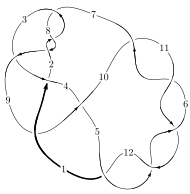
\includegraphics[width=112pt]{../../../GIT/diagram.site/Diagrams/png/1940_12a_1139.png}\\
\ \ \ A knot diagram\footnotemark}&
\allowdisplaybreaks
\textbf{Linearized knot diagam} \\
\cline{2-2}
 &
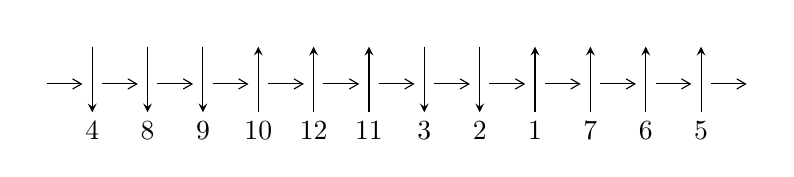
\begin{tikzpicture}[x=20pt, y=17pt]
	% nodes
	\node (C0) at (0, 0) {};
	\node (C1) at (1, 0) {};
	\node (C1U) at (1, +1) {};
	\node (C1D) at (1, -1) {4};

	\node (C2) at (2, 0) {};
	\node (C2U) at (2, +1) {};
	\node (C2D) at (2, -1) {8};

	\node (C3) at (3, 0) {};
	\node (C3U) at (3, +1) {};
	\node (C3D) at (3, -1) {9};

	\node (C4) at (4, 0) {};
	\node (C4U) at (4, +1) {};
	\node (C4D) at (4, -1) {10};

	\node (C5) at (5, 0) {};
	\node (C5U) at (5, +1) {};
	\node (C5D) at (5, -1) {12};

	\node (C6) at (6, 0) {};
	\node (C6U) at (6, +1) {};
	\node (C6D) at (6, -1) {11};

	\node (C7) at (7, 0) {};
	\node (C7U) at (7, +1) {};
	\node (C7D) at (7, -1) {3};

	\node (C8) at (8, 0) {};
	\node (C8U) at (8, +1) {};
	\node (C8D) at (8, -1) {2};

	\node (C9) at (9, 0) {};
	\node (C9U) at (9, +1) {};
	\node (C9D) at (9, -1) {1};

	\node (C10) at (10, 0) {};
	\node (C10U) at (10, +1) {};
	\node (C10D) at (10, -1) {7};

	\node (C11) at (11, 0) {};
	\node (C11U) at (11, +1) {};
	\node (C11D) at (11, -1) {6};

	\node (C12) at (12, 0) {};
	\node (C12U) at (12, +1) {};
	\node (C12D) at (12, -1) {5};
	\node (C13) at (13, 0) {};

	% arrows
	\draw[->,>={angle 60}]
	(C0) edge (C1) (C1) edge (C2) (C2) edge (C3) (C3) edge (C4) (C4) edge (C5) (C5) edge (C6) (C6) edge (C7) (C7) edge (C8) (C8) edge (C9) (C9) edge (C10) (C10) edge (C11) (C11) edge (C12) (C12) edge (C13) ;	\draw[->,>=stealth]
	(C1U) edge (C1D) (C2U) edge (C2D) (C3U) edge (C3D) (C4D) edge (C4U) (C5D) edge (C5U) (C6D) edge (C6U) (C7U) edge (C7D) (C8U) edge (C8D) (C9D) edge (C9U) (C10D) edge (C10U) (C11D) edge (C11U) (C12D) edge (C12U) ;
	\end{tikzpicture} \\
\hhline{~~} \\& 
\textbf{Solving Sequence} \\ \cline{2-2} 
 &
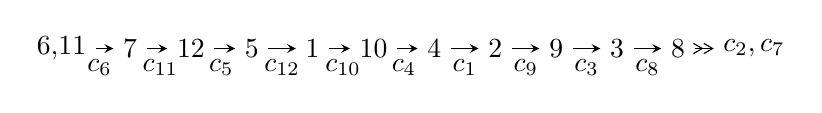
\begin{tikzpicture}[x=22pt, y=7pt]
	% node
	\node (A0) at (-1/8, 0) {6,11};
	\node (A1) at (1, 0) {7};
	\node (A2) at (2, 0) {12};
	\node (A3) at (3, 0) {5};
	\node (A4) at (4, 0) {1};
	\node (A5) at (5, 0) {10};
	\node (A6) at (6, 0) {4};
	\node (A7) at (7, 0) {2};
	\node (A8) at (8, 0) {9};
	\node (A9) at (9, 0) {3};
	\node (A10) at (10, 0) {8};
	\node (C1) at (1/2, -1) {$c_{6}$};
	\node (C2) at (3/2, -1) {$c_{11}$};
	\node (C3) at (5/2, -1) {$c_{5}$};
	\node (C4) at (7/2, -1) {$c_{12}$};
	\node (C5) at (9/2, -1) {$c_{10}$};
	\node (C6) at (11/2, -1) {$c_{4}$};
	\node (C7) at (13/2, -1) {$c_{1}$};
	\node (C8) at (15/2, -1) {$c_{9}$};
	\node (C9) at (17/2, -1) {$c_{3}$};
	\node (C10) at (19/2, -1) {$c_{8}$};
	\node (A11) at (45/4, 0) {$c_{2},c_{7}$};

	% edge
	\draw[->,>=stealth]	
	(A0) edge (A1) (A1) edge (A2) (A2) edge (A3) (A3) edge (A4) (A4) edge (A5) (A5) edge (A6) (A6) edge (A7) (A7) edge (A8) (A8) edge (A9) (A9) edge (A10) ;
	\draw[->>,>={angle 60}]	
	(A10) edge (A11);
\end{tikzpicture} \\ 

\end{tabular} \\

\footnotetext{
The image of knot diagram is generated by the software ``\textbf{Draw programme}" developed by Andrew Bartholomew(\url{http://www.layer8.co.uk/maths/draw/index.htm\#Running-draw}), where we modified some parts for our purpose(\url{https://github.com/CATsTAILs/LinksPainter}).
}\phantom \\ \newline 
\centering \textbf{Ideals for irreducible components\footnotemark of $X_{\text{par}}$} 
 
\begin{align*}
I^u_{1}&=\langle 
u^{50}+u^{49}+\cdots+3 u+1\rangle \\
\\
\end{align*}
\raggedright * 1 irreducible components of $\dim_{\mathbb{C}}=0$, with total 50 representations.\\
\footnotetext{All coefficients of polynomials are rational numbers. But the coefficients are sometimes approximated in decimal forms when there is not enough margin.}
\newpage
\renewcommand{\arraystretch}{1}
\centering \section*{I. $I^u_{1}= \langle u^{50}+u^{49}+\cdots+3 u+1 \rangle$}
\flushleft \textbf{(i) Arc colorings}\\
\begin{tabular}{m{7pt} m{180pt} m{7pt} m{180pt} }
\flushright $a_{6}=$&$\begin{pmatrix}1\\0\end{pmatrix}$ \\
\flushright $a_{11}=$&$\begin{pmatrix}0\\u\end{pmatrix}$ \\
\flushright $a_{7}=$&$\begin{pmatrix}1\\- u^2\end{pmatrix}$ \\
\flushright $a_{12}=$&$\begin{pmatrix}u\\u\end{pmatrix}$ \\
\flushright $a_{5}=$&$\begin{pmatrix}u^2+1\\u^2\end{pmatrix}$ \\
\flushright $a_{1}=$&$\begin{pmatrix}u^3+2 u\\u^3+u\end{pmatrix}$ \\
\flushright $a_{10}=$&$\begin{pmatrix}- u\\u^3+u\end{pmatrix}$ \\
\flushright $a_{4}=$&$\begin{pmatrix}- u^6-3 u^4+1\\u^8+4 u^6+4 u^4+2 u^2\end{pmatrix}$ \\
\flushright $a_{2}=$&$\begin{pmatrix}- u^{17}-10 u^{15}-37 u^{13}-60 u^{11}-35 u^9+8 u^7+16 u^5+4 u^3+u\\u^{19}+11 u^{17}+48 u^{15}+107 u^{13}+133 u^{11}+95 u^9+34 u^7+2 u^5- u^3+u\end{pmatrix}$ \\
\flushright $a_{9}=$&$\begin{pmatrix}- u^9-6 u^7-11 u^5-6 u^3- u\\- u^9-5 u^7-7 u^5-2 u^3+u\end{pmatrix}$ \\
\flushright $a_{3}=$&$\begin{pmatrix}u^{26}+17 u^{24}+\cdots+u^2+1\\u^{26}+16 u^{24}+\cdots+6 u^4+u^2\end{pmatrix}$ \\
\flushright $a_{8}=$&$\begin{pmatrix}- u^{45}-28 u^{43}+\cdots-4 u^3- u\\u^{47}+29 u^{45}+\cdots-2 u^5+u\end{pmatrix}$\\&\end{tabular}
\flushleft \textbf{(ii) Obstruction class $= -1$}\\~\\
\flushleft \textbf{(iii) Cusp Shapes $= 4 u^{49}+4 u^{48}+\cdots+20 u+10$}\\~\\
\newpage\renewcommand{\arraystretch}{1}
\flushleft \textbf{(iv) u-Polynomials at the component}\newline \\
\begin{tabular}{m{50pt}|m{274pt}}
Crossings & \hspace{64pt}u-Polynomials at each crossing \\
\hline $$\begin{aligned}c_{1}\end{aligned}$$&$\begin{aligned}
&u^{50}-11 u^{49}+\cdots-971 u+99
\end{aligned}$\\
\hline $$\begin{aligned}c_{2},c_{7},c_{8}\end{aligned}$$&$\begin{aligned}
&u^{50}- u^{49}+\cdots- u+1
\end{aligned}$\\
\hline $$\begin{aligned}c_{3}\end{aligned}$$&$\begin{aligned}
&u^{50}+u^{49}+\cdots-3 u+1
\end{aligned}$\\
\hline $$\begin{aligned}c_{4}\end{aligned}$$&$\begin{aligned}
&u^{50}- u^{49}+\cdots+135 u+29
\end{aligned}$\\
\hline $$\begin{aligned}c_{5},c_{6},c_{10}\\c_{11},c_{12}\end{aligned}$$&$\begin{aligned}
&u^{50}- u^{49}+\cdots-3 u+1
\end{aligned}$\\
\hline $$\begin{aligned}c_{9}\end{aligned}$$&$\begin{aligned}
&u^{50}-7 u^{49}+\cdots-511 u+215
\end{aligned}$\\
\hline
\end{tabular}\\~\\
\newpage\renewcommand{\arraystretch}{1}
\flushleft \textbf{(v) Riley Polynomials at the component}\newline \\
\begin{tabular}{m{50pt}|m{274pt}}
Crossings & \hspace{64pt}Riley Polynomials at each crossing \\
\hline $$\begin{aligned}c_{1}\end{aligned}$$&$\begin{aligned}
&y^{50}+13 y^{49}+\cdots+182789 y+9801
\end{aligned}$\\
\hline $$\begin{aligned}c_{2},c_{7},c_{8}\end{aligned}$$&$\begin{aligned}
&y^{50}+45 y^{49}+\cdots+y+1
\end{aligned}$\\
\hline $$\begin{aligned}c_{3}\end{aligned}$$&$\begin{aligned}
&y^{50}+y^{49}+\cdots+y+1
\end{aligned}$\\
\hline $$\begin{aligned}c_{4}\end{aligned}$$&$\begin{aligned}
&y^{50}+9 y^{49}+\cdots-5523 y+841
\end{aligned}$\\
\hline $$\begin{aligned}c_{5},c_{6},c_{10}\\c_{11},c_{12}\end{aligned}$$&$\begin{aligned}
&y^{50}+65 y^{49}+\cdots+y+1
\end{aligned}$\\
\hline $$\begin{aligned}c_{9}\end{aligned}$$&$\begin{aligned}
&y^{50}+17 y^{49}+\cdots+738629 y+46225
\end{aligned}$\\
\hline
\end{tabular}\\~\\
\newpage\flushleft \textbf{(vi) Complex Volumes and Cusp Shapes}
$$\begin{array}{c|c|c}  
\text{Solutions to }I^u_{1}& \I (\text{vol} + \sqrt{-1}CS) & \text{Cusp shape}\\
 \hline 
\begin{aligned}
u &= -0.267263 + 0.974653 I\end{aligned}
 & -2.52565 - 3.29260 I & \phantom{-0.000000 } 0 \\ \hline\begin{aligned}
u &= -0.267263 - 0.974653 I\end{aligned}
 & -2.52565 + 3.29260 I & \phantom{-0.000000 } 0 \\ \hline\begin{aligned}
u &= \phantom{-}0.300039 + 0.917172 I\end{aligned}
 & \phantom{-}3.68092 + 1.88018 I & \phantom{-}3.28403 - 3.42848 I \\ \hline\begin{aligned}
u &= \phantom{-}0.300039 - 0.917172 I\end{aligned}
 & \phantom{-}3.68092 - 1.88018 I & \phantom{-}3.28403 + 3.42848 I \\ \hline\begin{aligned}
u &= \phantom{-}0.303413 + 0.993489 I\end{aligned}
 & -3.97531 + 7.01696 I & \phantom{-0.000000 } 0 \\ \hline\begin{aligned}
u &= \phantom{-}0.303413 - 0.993489 I\end{aligned}
 & -3.97531 - 7.01696 I & \phantom{-0.000000 } 0 \\ \hline\begin{aligned}
u &= -0.228796 + 1.014910 I\end{aligned}
 & -2.85501 - 3.56952 I & \phantom{-0.000000 } 0 \\ \hline\begin{aligned}
u &= -0.228796 - 1.014910 I\end{aligned}
 & -2.85501 + 3.56952 I & \phantom{-0.000000 } 0 \\ \hline\begin{aligned}
u &= \phantom{-}0.167253 + 1.029960 I\end{aligned}
 & -5.48280 + 0.26480 I & \phantom{-0.000000 } 0 \\ \hline\begin{aligned}
u &= \phantom{-}0.167253 - 1.029960 I\end{aligned}
 & -5.48280 - 0.26480 I & \phantom{-0.000000 } 0 \\ \hline\begin{aligned}
u &= -0.322805 + 0.992607 I\end{aligned}
 & \phantom{-}1.41582 - 10.58410 I & \phantom{-0.000000 } 0 \\ \hline\begin{aligned}
u &= -0.322805 - 0.992607 I\end{aligned}
 & \phantom{-}1.41582 + 10.58410 I & \phantom{-0.000000 } 0 \\ \hline\begin{aligned}
u &= -0.122951 + 1.057210 I\end{aligned}
 & -0.72813 + 3.07389 I & \phantom{-0.000000 } 0 \\ \hline\begin{aligned}
u &= -0.122951 - 1.057210 I\end{aligned}
 & -0.72813 - 3.07389 I & \phantom{-0.000000 } 0 \\ \hline\begin{aligned}
u &= \phantom{-}0.293582 + 0.669845 I\end{aligned}
 & \phantom{-}5.06450 + 3.76743 I & \phantom{-}4.59609 - 5.34956 I \\ \hline\begin{aligned}
u &= \phantom{-}0.293582 - 0.669845 I\end{aligned}
 & \phantom{-}5.06450 - 3.76743 I & \phantom{-}4.59609 + 5.34956 I \\ \hline\begin{aligned}
u &= -0.165448 + 0.666519 I\end{aligned}
 & -0.48337 - 1.40800 I & \phantom{-}0.29896 + 5.97525 I \\ \hline\begin{aligned}
u &= -0.165448 - 0.666519 I\end{aligned}
 & -0.48337 + 1.40800 I & \phantom{-}0.29896 - 5.97525 I \\ \hline\begin{aligned}
u &= -0.376224 + 0.489617 I\end{aligned}
 & \phantom{-}4.12836 + 4.50612 I & \phantom{-}3.44574 - 0.89848 I \\ \hline\begin{aligned}
u &= -0.376224 - 0.489617 I\end{aligned}
 & \phantom{-}4.12836 - 4.50612 I & \phantom{-}3.44574 + 0.89848 I \\ \hline\begin{aligned}
u &= -0.543737 + 0.197520 I\end{aligned}
 & \phantom{-}5.08510 - 7.63642 I & \phantom{-}6.10437 + 7.49857 I \\ \hline\begin{aligned}
u &= -0.543737 - 0.197520 I\end{aligned}
 & \phantom{-}5.08510 + 7.63642 I & \phantom{-}6.10437 - 7.49857 I \\ \hline\begin{aligned}
u &= \phantom{-}0.513985 + 0.202878 I\end{aligned}
 & -0.28571 + 4.22898 I & \phantom{-}1.46755 - 7.80159 I \\ \hline\begin{aligned}
u &= \phantom{-}0.513985 - 0.202878 I\end{aligned}
 & -0.28571 - 4.22898 I & \phantom{-}1.46755 + 7.80159 I \\ \hline\begin{aligned}
u &= \phantom{-}0.334706 + 0.422369 I\end{aligned}
 & -1.09545 - 1.33004 I & -1.86370 + 0.68284 I \\ \hline\begin{aligned}
u &= \phantom{-}0.334706 - 0.422369 I\end{aligned}
 & -1.09545 + 1.33004 I & -1.86370 - 0.68284 I \\ \hline\begin{aligned}
u &= \phantom{-}0.521502 + 0.099632 I\end{aligned}
 & \phantom{-}6.77978 - 0.91733 I & \phantom{-}9.49995 - 0.90455 I \\ \hline\begin{aligned}
u &= \phantom{-}0.521502 - 0.099632 I\end{aligned}
 & \phantom{-}6.77978 + 0.91733 I & \phantom{-}9.49995 + 0.90455 I \\ \hline\begin{aligned}
u &= -0.420230 + 0.281296 I\end{aligned}
 & \phantom{-}1.13900 - 1.36467 I & \phantom{-}1.97434 + 4.92900 I \\ \hline\begin{aligned}
u &= -0.420230 - 0.281296 I\end{aligned}
 & \phantom{-}1.13900 + 1.36467 I & \phantom{-}1.97434 - 4.92900 I\\
 \hline 
 \end{array}$$\newpage$$\begin{array}{c|c|c}  
\text{Solutions to }I^u_{1}& \I (\text{vol} + \sqrt{-1}CS) & \text{Cusp shape}\\
 \hline 
\begin{aligned}
u &= -0.448171 + 0.153855 I\end{aligned}
 & \phantom{-}0.966748 - 0.838351 I & \phantom{-}5.97312 + 2.21174 I \\ \hline\begin{aligned}
u &= -0.448171 - 0.153855 I\end{aligned}
 & \phantom{-}0.966748 + 0.838351 I & \phantom{-}5.97312 - 2.21174 I \\ \hline\begin{aligned}
u &= \phantom{-}0.02262 + 1.64150 I\end{aligned}
 & -2.97025 + 4.57226 I & \phantom{-0.000000 } 0 \\ \hline\begin{aligned}
u &= \phantom{-}0.02262 - 1.64150 I\end{aligned}
 & -2.97025 - 4.57226 I & \phantom{-0.000000 } 0 \\ \hline\begin{aligned}
u &= -0.01192 + 1.65807 I\end{aligned}
 & -8.80943 - 1.80374 I & \phantom{-0.000000 } 0 \\ \hline\begin{aligned}
u &= -0.01192 - 1.65807 I\end{aligned}
 & -8.80943 + 1.80374 I & \phantom{-0.000000 } 0 \\ \hline\begin{aligned}
u &= \phantom{-}0.07257 + 1.69685 I\end{aligned}
 & -5.55279 + 3.30682 I & \phantom{-0.000000 } 0 \\ \hline\begin{aligned}
u &= \phantom{-}0.07257 - 1.69685 I\end{aligned}
 & -5.55279 - 3.30682 I & \phantom{-0.000000 } 0 \\ \hline\begin{aligned}
u &= -0.06955 + 1.71380 I\end{aligned}
 & -12.07900 - 4.64056 I & \phantom{-0.000000 } 0 \\ \hline\begin{aligned}
u &= -0.06955 - 1.71380 I\end{aligned}
 & -12.07900 + 4.64056 I & \phantom{-0.000000 } 0 \\ \hline\begin{aligned}
u &= -0.08449 + 1.71651 I\end{aligned}
 & -8.1767 - 12.2216 I & \phantom{-0.000000 } 0 \\ \hline\begin{aligned}
u &= -0.08449 - 1.71651 I\end{aligned}
 & -8.1767 + 12.2216 I & \phantom{-0.000000 } 0 \\ \hline\begin{aligned}
u &= \phantom{-}0.07899 + 1.71722 I\end{aligned}
 & -13.5884 + 8.5544 I & \phantom{-0.000000 } 0 \\ \hline\begin{aligned}
u &= \phantom{-}0.07899 - 1.71722 I\end{aligned}
 & -13.5884 - 8.5544 I & \phantom{-0.000000 } 0 \\ \hline\begin{aligned}
u &= -0.05785 + 1.72253 I\end{aligned}
 & -12.61190 - 4.72463 I & \phantom{-0.000000 } 0 \\ \hline\begin{aligned}
u &= -0.05785 - 1.72253 I\end{aligned}
 & -12.61190 + 4.72463 I & \phantom{-0.000000 } 0 \\ \hline\begin{aligned}
u &= \phantom{-}0.04441 + 1.72496 I\end{aligned}
 & -15.3216 + 1.1374 I & \phantom{-0.000000 } 0 \\ \hline\begin{aligned}
u &= \phantom{-}0.04441 - 1.72496 I\end{aligned}
 & -15.3216 - 1.1374 I & \phantom{-0.000000 } 0 \\ \hline\begin{aligned}
u &= -0.03365 + 1.72806 I\end{aligned}
 & -10.67560 + 2.41850 I & \phantom{-0.000000 } 0 \\ \hline\begin{aligned}
u &= -0.03365 - 1.72806 I\end{aligned}
 & -10.67560 - 2.41850 I & \phantom{-0.000000 } 0\\
 \hline 
 \end{array}$$\newpage
\newpage\renewcommand{\arraystretch}{1}
\centering \section*{ II. u-Polynomials}
\begin{tabular}{m{50pt}|m{274pt}}
Crossings & \hspace{64pt}u-Polynomials at each crossing \\
\hline $$\begin{aligned}c_{1}\end{aligned}$$&$\begin{aligned}
&u^{50}-11 u^{49}+\cdots-971 u+99
\end{aligned}$\\
\hline $$\begin{aligned}c_{2},c_{7},c_{8}\end{aligned}$$&$\begin{aligned}
&u^{50}- u^{49}+\cdots- u+1
\end{aligned}$\\
\hline $$\begin{aligned}c_{3}\end{aligned}$$&$\begin{aligned}
&u^{50}+u^{49}+\cdots-3 u+1
\end{aligned}$\\
\hline $$\begin{aligned}c_{4}\end{aligned}$$&$\begin{aligned}
&u^{50}- u^{49}+\cdots+135 u+29
\end{aligned}$\\
\hline $$\begin{aligned}c_{5},c_{6},c_{10}\\c_{11},c_{12}\end{aligned}$$&$\begin{aligned}
&u^{50}- u^{49}+\cdots-3 u+1
\end{aligned}$\\
\hline $$\begin{aligned}c_{9}\end{aligned}$$&$\begin{aligned}
&u^{50}-7 u^{49}+\cdots-511 u+215
\end{aligned}$\\
\hline
\end{tabular}\newpage\renewcommand{\arraystretch}{1}
\centering \section*{ III. Riley Polynomials}
\begin{tabular}{m{50pt}|m{274pt}}
Crossings & \hspace{64pt}Riley Polynomials at each crossing \\
\hline $$\begin{aligned}c_{1}\end{aligned}$$&$\begin{aligned}
&y^{50}+13 y^{49}+\cdots+182789 y+9801
\end{aligned}$\\
\hline $$\begin{aligned}c_{2},c_{7},c_{8}\end{aligned}$$&$\begin{aligned}
&y^{50}+45 y^{49}+\cdots+y+1
\end{aligned}$\\
\hline $$\begin{aligned}c_{3}\end{aligned}$$&$\begin{aligned}
&y^{50}+y^{49}+\cdots+y+1
\end{aligned}$\\
\hline $$\begin{aligned}c_{4}\end{aligned}$$&$\begin{aligned}
&y^{50}+9 y^{49}+\cdots-5523 y+841
\end{aligned}$\\
\hline $$\begin{aligned}c_{5},c_{6},c_{10}\\c_{11},c_{12}\end{aligned}$$&$\begin{aligned}
&y^{50}+65 y^{49}+\cdots+y+1
\end{aligned}$\\
\hline $$\begin{aligned}c_{9}\end{aligned}$$&$\begin{aligned}
&y^{50}+17 y^{49}+\cdots+738629 y+46225
\end{aligned}$\\
\hline
\end{tabular}
\vskip 2pc
\end{document}